\subsection{Architettura dei simulatori} \label{sec:architettura_simulatori}
Nonostante i simulatori non siano ufficialmente considerati come parte fondamentale del prodotto dalla proponente, ma necessari solamente per dimostrare il corretto funzionamento del sistema, il nostro team ha comunque scelto di dedicare alcune risorse alla progettazione di questa componente nell'ambito del progetto didattico.

Inoltre, abbiamo deciso di implementare e tenere conto delle possibili logiche dei microcontrollori associati ai sensori IoT, che possono effettuare operazioni per rendere più efficiente l'intero sistema.

Nei paragrafi successivi, verrà presentata l'architettura individuata mediante l'utilizzo di diagrammi delle classi e relative descrizioni. Inoltre, saranno motivate le scelte dei design pattern individuati e le decisioni progettuali rilevanti. Successivamente, per ogni classe, saranno illustrati metodi e attributi.

\subsubsection{Modulo simulatori sensori}
\begin{figure}[H]
    \centering
    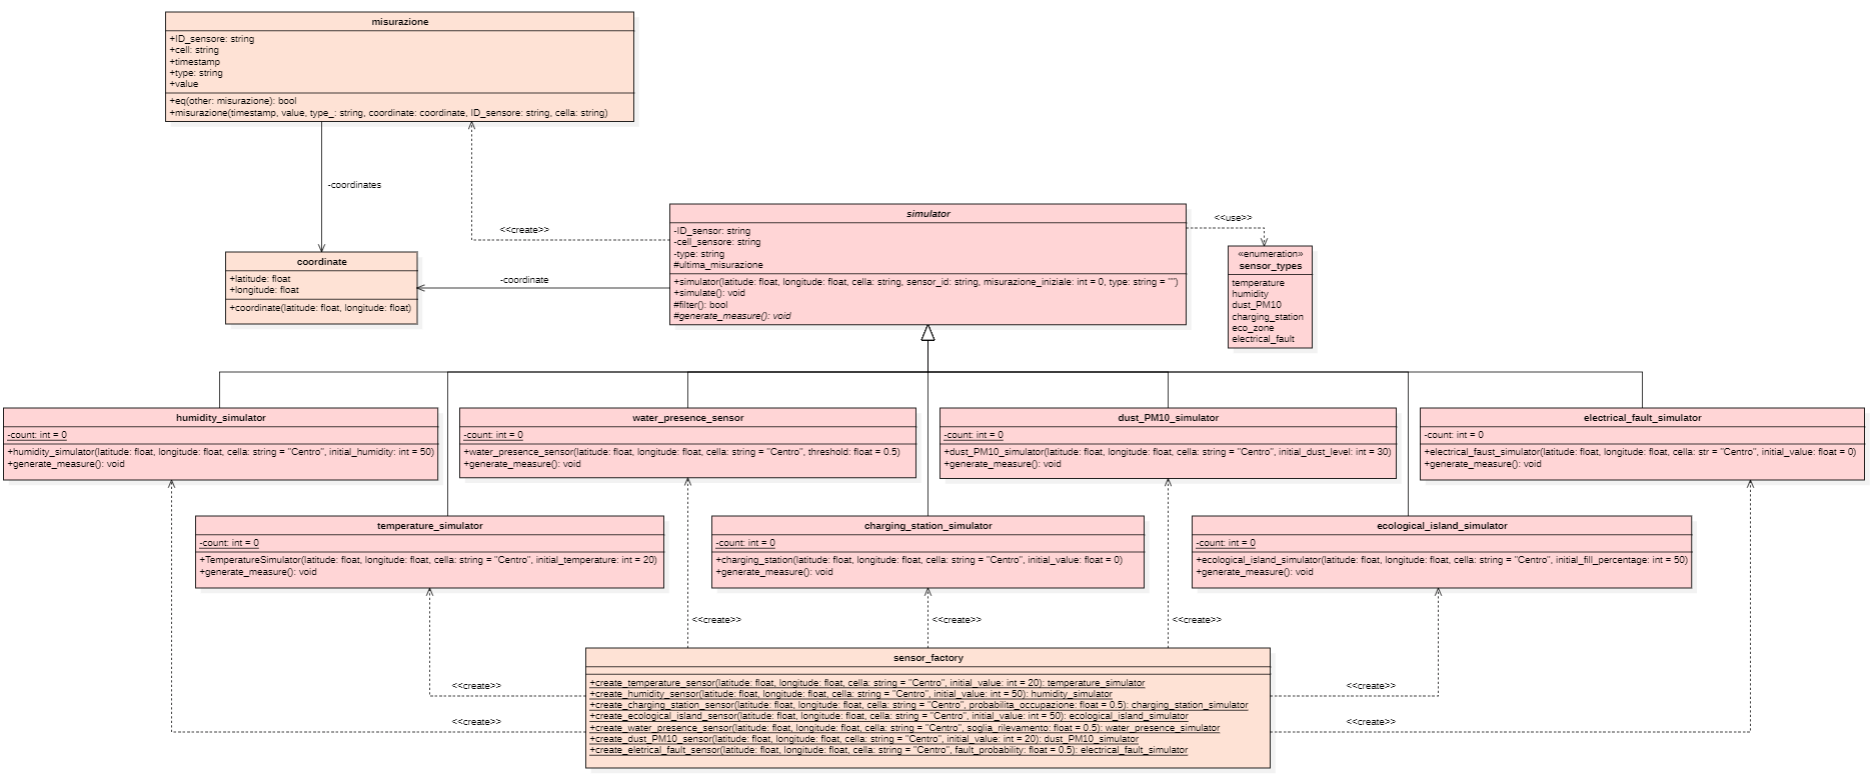
\includegraphics[width=1.1\textwidth]{../Images/SpecificaTecnica/simulatoriSensori.PNG}
    \caption{Modulo simulatori sensori - InnovaCity}
    \label{fig: Modulo_simulatori_sensori}
\end{figure}
Questo modulo si occupa della generazione di dati per diverse tipologie di sensori.
In particolare sono stati implementati simulatori per i seguenti tipi di sensori:
\begin{itemize}
    \item Sensori di temperatura;
    \item Sensori di umidità;
    \item Sensori di polveri sottili PM10;
    \item Sensori di stato occupazione colonnine di ricarica;
    \item Sensori di stato riempimento isole ecologiche;
    \item Sensori di presenza d'acqua;
    \item Sensori di guasto elettrico.
\end{itemize}
\paragraph{Design pattern Template Method} \label{sec:templateSIM}

La classe astratta \textit{simulator} implementa il design pattern \textit{Template Method}. Il metodo \textit{simulate()} fornisce lo scheletro dell'algoritmo per la generazione delle misurazioni e non può essere ridefinito nelle implementatazioni. Le classi che estendono \textit{simulator} implementano i metodi:
\begin{itemize}
    \item \textbf{\textit{generate\_measure()}:} Per la generazione semi-randomica della misurazione associata al tipo di sensore, di fatto non è richiesta una generazione di misurazioni realistiche dal prodotto, ma per poter avere una visualizzazione finale delle misurazioni non altalenanti ogni misurazione viene generata sulla base di quella precedente con una variazione limitata;
    
    \item \textbf{\textit{adapt()} - "hook method":} L'implementazione di default non modifica in alcun modo la misurazione generata. Può essere ridefinito per implementare la logica di adattamento della misurazione.
    
    Ad esempio:
    \begin{itemize}
        \item Per i sensori di polveri sottili PM10, la misurazione può essere adattata cambiando il valore dell'unità di misura µg/m³ in mg/m³ senza modifcare la logica di generazione in \textit{generate\_measure()};
        
        \item Per i sensori di temperatura, la misurazione può essere adattata cambiando il valore dell'unità di misura da °C a Fahrenheit  senza modifcare la logica di generazione in \textit{generate\_measure()};
        
        ~•~ Fahrenheit = (Celsius × 9/5) + 32
 
        \item Questo apre le porte alla possibilità di creare per una stessa tipoligia di sensore diverse implementazioni, che generano misurazioni con unità di misura diverse, senza dover modificare la logica di generazione che dichiara l'unità di misura generata di default, ma semplicemente estendendo la classe e ridefinendo il metodo \textit{adapt()} inserendo la formula di trasformazione.
        
    \end{itemize}
    \item Per garantire il rispetto del \textbf{Liskov Substitution Principle (LSP)} \textit{"Objects of a superclass should be replaceable with objects of its subtypes without altering the program's correctness."}:
    \begin{itemize}
        \item Il metodo \textit{adapt()} si limita a convertire le misurazioni senza alterare il comportamento generale del metodo \textit{simulate()} e senza modificare il tipo della misurazione generata da \textit{generate\_measure()};
        
        \item Il metodo \textit{generate\_measure()} viene reso \textbf{final} nelle concretizzazioni di \textit{simulator} impedendo la ridefinizione del comportamento.
    \end{itemize}

    In generale le postcondizioni sono piu forti nelle classi derivate, mentre non variano le precondizioni garantendo il rispetto di \textit{LSP}.
    
    Ad esempio:

    \begin{itemize}
        \item In \textit{simulator}:

        \begin{itemize}
            \item La postcondizione del metodo \textit{simulate()} in simulator è la generazione di un oggetto di tipo \textit{misurazione};
            
            \item La postcondizione del metodo \textit{generate\_measure} è la generazione del valore della misurazione.
            
            \item La postcondizione del metodo \textit{adapt()} è la possibilità di convertire il valore della misurazione.
        \end{itemize}

        \item In \textit{temperature\_simulator}, che eredita da \textit{simulator}:
        \begin{itemize}
            \item La postcondizione del metodo \textit{simulate()} è la generazione di un oggetto di tipo \textit{misurazione} di temperatura;
            
            \item La postcondizione del metodo \textit{generate\_measure} è la generazione del valore di una misurazione di temperatura;
            
            \item La postcondizione del metodo \textit{adapt()} è la possibilità di convertire il valore della misurazione ad un altra unità di misura (Kelvin, Fahrenheit).
        \end{itemize}

        \item In una possibile estensione futura \textit{temperature\_simulator\_fahrenheit}, che eredita da \textit{temperature\_simulator}:
        \begin{itemize}
            \item La postcondizione del metodo \textit{simulate()} è la generazione di un oggetto di tipo \textit{misurazione} di temperatura espresso in gradi Fahrenheit;
            
            \item La postcondizione del metodo \textit{generate\_measure} rimane invariata;
            
            \item La postcondizione del metodo \textit{adapt()} è di convertire il valore della misurazione dall'unità di misura di default a Fahrenheit.
        \end{itemize}
    \end{itemize}
\end{itemize}

Al termine delle operazioni di generazione e adattamento, il metodo \textit{simulate()} crea e restituisce un oggetto di tipo \textit{misurazione}.

Il design pattern \textit{Template Method} è stato scelto per:
\begin{itemize}
    \item Permettere una facile estensione del sistema con nuovi tipi di sensori che dovranno unicamente implementare la loro logica di generazione delle misurazioni e di adapting se necessario;
    
    \item Standardizzare i passi per la generazione delle misurazioni, garantendo coerenza e manutenibilità del codice;
    
    \item Ridurre la duplicazione del codice.
\end{itemize}

Come già esposto, una volta ottenuto lo stato del sensore, esso viene inserito in un oggetto di tipo \textit{misurazione}. Questo oggetto contiene informazioni di contesto come:
\begin{itemize}
    \item Identificativo del sensore;
    \item Cella della città in cui è presente il sensore;
    \item Timestamp della misurazione;
    \item Valore della misurazione;
    \item Coordinate;
    \item Tipologia di misurazione.
\end{itemize}

L'oggetto \textit{misurazione} viene poi ritornato al chiamante che si occuperà di inviarlo al server Kafka.
Un oggetto di tipo \textit{simulator} infatti, verrà assegnato ad ogni \textit{simulator\_thread}. Esso chiamerà ad intervalli regolari il metodo \textit{simulate()} ottenendo appunto la misurazione che invierà poi al server Kafka tramite un modulo apposito e indipendendente.

\paragraph{Design pattern Factory}
sensor\_factory implementa il design pattern \textit{Factory} per la creazione di simulatori dei sensori.
Il pattern \textit{Factory} è un pattern di tipo “Creazionale” secondo la classificazione della GoF.

I pattern di tipo creazionali si occupano della costruzione delle simulazioni dei sensori e delle problematiche che si possono originare, astraggono il processo di creazione degli oggetti, nascondono i dettagli della creazione e rendono i sistemi indipendenti da come gli oggetti sono creati e composti.

Il pattern \textit{Factory} incapsula la creazione concreta dei sensori, consentendo al client
(l’utilizzatore) di non conoscere i dettagli.

\paragraph{Classi, interfacce metodi e attributi:}
\begin{itemize}
    \item {\textbf{Classe astratta: \textit{simulator}}}
    \begin{itemize}
        \item \textbf{Attributi}: 
        \begin{itemize}
            \item \textbf{ID\_sensor: string [private]} - Identificatore univoco del sensore.
            \item \textbf{cella\_sensore: string [private]} - Identificatore della cella del sensore.
            \item \textbf{coordinate: coordinate [private]} - Coordinate geografiche del sensore.
            \item \textbf{misurazione: T [protected]} - Misurazione corrente del sensore.
            \item \textbf{type: string [private]} - Tipo di sensore.
        \end{itemize}
        \item \textbf{Metodi}:
        \begin{itemize}
            \item \textbf{simulate(): misurazione [public]} - Metodo principale per simulare la generazione di una misurazione.
            \item 
            Si basa sul design pattern Template Method:
            \begin{enumerate}
                \item Chiama generate\_measure() per generare un valore di misurazione.
                \item Chiama adapt() per effettuare adattamenti se necessari.
                \item Restituisce un oggetto \textit{misurazione} con data e ora corrente, valore misurato, tipo di sensore, coordinate e identificativo del sensore.
            \end{enumerate}
            \item \textbf{generate\_measure(): None [protected]} - Metodo astratto da implementare nelle classi concrete per generare un valore di misurazione semi-casuale coerente con la tipolgia di sensore da salvare nell'attributo \textit{misurazione}.
            \item \textbf{adapt(): void [protected]} - Fornisce un'implementazione di default che non modifica in alcun modo la misurazione generata. Può essere ridefinito per implementare la logica di adattamento della misurazione come conversioni di unità di misura.
        \end{itemize}
        \item \textbf{Note}:
        \begin{itemize}
            \item La classe \textit{simulator} è astratta e definisce il comportamento generale della simulazione della misurazione, pattern \textit{Template method}.
            \item Le classi concrete che ereditano da \textit{simulator} devono implementare il metodo astratto generate\_measure().
            \item Il metodo adapt() può essere ridefinito nelle classi concrete per implementare conversioni o adattamenti necessari.
            \item Il metodo \textit{simulate()} è final e non può essere ridefinito.
            \item Spiegazioni esaustive sono state presentate in: \ref{sec:templateSIM}
        \end{itemize}
    \end{itemize}
        
    \item{\textbf{Enumerazione: \textit{sensor\_types}}}
    \begin{itemize}
        \item \textbf{Costanti}: 
        \begin{itemize}
            \item \textbf{TEMPERATURE: string [public]} - Rappresenta la nomenclatura dei sensore di temperatura.
            \item \textbf{HUMIDITY: string [public]} - Rappresenta la nomenclatura dei sensore di umidità.
            \item \textbf{DUST\_PM10: string [public]} - Rappresenta la nomenclatura dei sensore di "polvere PM10".
            \item \textbf{CHARGING\_STATION: string [public]} - Rappresenta la nomenclatura dei sensore di stato delle colonnine di ricarica.
            \item \textbf{ECOLOGICAL\_ISLAND: string [public]} - Rappresenta la nomenclatura dei sensore di stato riempimento isole ecologica.
            \item \textbf{WATER\_PRESENCE: string [public]} - Rappresenta la nomenclatura dei sensore di presenza d'acqua.
            \item \textbf{ELECTRICAL\_FAULT: string [public]} - Rappresenta la nomenclatura dei sensore di guasti elettrici.
        \end{itemize}

        \item \textbf{Note}:
        \begin{itemize}
            \item L'enumerazione viene utilizzata per centralizzare la gestione della nomenclatura dei tipi di sensori che verrà salvata nelle misurazioni.
        \end{itemize}
    \end{itemize}
        
    \item{\textbf{Classe: \textit{temperature\_simulator}}}
    \begin{itemize}
        \item \textbf{Attributi:}
        \begin{itemize}
            \item \textbf{count: int [private, static]} - Contatore statico per generare un ID univoco per ogni istanza.
        \end{itemize}
        \item\textbf{Metodi}: 
        \begin{itemize}
            \item \textbf{generate\_measure(): None [protected,final]} - Genera una misurazione di temperatura in gradi Celsius semi-casuale e aggiorna lo stato interno con il valore della misurazione corrente.
        \end{itemize}
        \item\textbf{Note}:
        \begin{itemize}
            \item La classe \textit{temperature\_simulator} è una classe concreta che eredita dalla classe astratta \textit{simulator}.
            \item Il costruttore genera automaticamente un ID sensore univoco per ogni istanza.
            \item Dichiara di generare misurazioni di temperatura con unità di default (Gradi Celsius), possibili classi derivate possono effettuare conversioni ad altre unità di misura (Kelvin,Fahrenheit) tramite il metodo \textit{adapt()}, senza dover modificare la logica di generazione.
        \end{itemize}
    \end{itemize}
    
    \item{\textbf{Classe: \textit{humidity\_simulator}}}
    \begin{itemize}
        \item\textbf{Attributi:}
        \begin{itemize}
            \item \textbf{count: int [private, static]} - Contatore statico per generare un ID univoco per ogni istanza.
        \end{itemize}
        \item \textbf{Metodi}: 
        \begin{itemize}
            \item \textbf{generate\_measure(): None [protected,final]} - Genera una misurazione di umidità in percentuale semi-casuale e aggiorna lo stato interno con il valore della misurazione corrente.
        \end{itemize}
        \item \textbf{Note}:
        \begin{itemize}
        \item La classe \textit{humidity\_simulator} è una classe concreta che eredita dalla classe astratta \textit{simulator}.
        \item Il costruttore genera automaticamente un ID sensore univoco per ogni istanza.
        \item Dichiara di generare misurazioni di umidità con unità di default (Percentuale), possibili classi derivate possono effettuare conversioni ad altre unità di misura (g/m³) tramite il metodo \textit{adapt()}, senza dover modificare la logica di generazione.
        \end{itemize}
    \end{itemize}

    \item{\textbf{Classe: \textit{charging\_station\_simulator}}}
    \begin{itemize}
        \item \textbf{Attributi}: 
        \begin{itemize}
            \item \textbf{count: int [private, static]} - Contatore statico per generare un ID univoco per ogni istanza.
        \end{itemize}
        \item \textbf{Metodi}:
        \begin{itemize}
            \item \textbf{generate\_measure(): None [protected,final]} - Genera lo stato della colonnina di ricarica (Occupato: \textsc{True}, Libero: \textsc{False}) basata su una probabilità di transizione e aggiorna lo stato interno con il valore della misurazione corrente.
        \end{itemize}
        \item \textbf{Note}:
        \begin{itemize}
            \item La classe \textit{charging\_station\_simulator} è una classe concreta che eredita dalla classe astratta \textit{simulator}.
            \item Il costruttore genera automaticamente un ID sensore univoco per ogni istanza.
            \item Implementa il metodo astratto \textit{generate\_measure()} per generare una misurazione basata sulla probabilità di transizione.
        \end{itemize}
    \end{itemize}

    \item{\textbf{Classe: \textit{dust\_PM10\_simulator}}}
    \begin{itemize}
        \item \textbf{Attributi}: 
        \begin{itemize}
            \item \textbf{count: int [private, static]} - Contatore statico per generare un ID univoco per ogni istanza.
        \end{itemize}
        \item \textbf{Metodi}: 
        \begin{itemize}
            \item \textbf{generate\_measure(): None [protected,final]} - Genera una variazione di quantità di polvere PM10 semi-casuale e aggiorna lo stato interno con il valore della misurazione corrente.
        \end{itemize}
        \item \textbf{Note}:
        \begin{itemize}
            \item La classe \textit{dust\_PM10\_simulator} è una classe concreta che eredita dalla classe astratta \textit{simulator}.
            \item Il costruttore genera automaticamente un ID sensore univoco per ogni istanza.
            \item Dichiara di generare misurazioni di polvere PM10 in con unità di default (µg/m³), possibili classi derivate possono effettuare conversioni ad altre unità di misura (mg/m³) tramite il metodo \textit{adapt()}, senza dover modificare la logica di generazione.
        \end{itemize}
    \end{itemize}

    \item{\textbf{Classe: \textit{electrical\_fault\_simulator}}}
    \begin{itemize}
        \item \textbf{Attributi}: 
        \begin{itemize}
            \item \textbf{count: int [private, static]} - Contatore statico per generare un ID univoco per ogni istanza.
        \end{itemize}
        \item \textbf{Metodi}: 
        \begin{itemize}
            \item \textbf{generate\_measure(): None [protected,final]} - Genera lo stato di una centralina elettrica (Guasto verificato: \textsc{True}, Operativa: \textsc{False}) basandosi su una probabilità di guasto e aggiorna lo stato interno con il valore della misurazione corrente.
        \end{itemize}
        \item \textbf{Note}:
        \begin{itemize}
            \item La classe \textit{electrical\_fault\_simulator} è una classe concreta che eredita dalla classe astratta \textit{simulator}.
            \item Il costruttore genera automaticamente un ID sensore univoco per ogni istanza.
        \end{itemize}
    \end{itemize}

    \item{\textbf{Classe: \textit{ecological\_island\_simulator}}}
    \begin{itemize}
        \item \textbf{Attributi}: 
        \begin{itemize}
            \item \textbf{count: int [private, static]} - Contatore statico per generare un ID univoco per ogni istanza.
        \end{itemize}
        \item \textbf{Metodi}: 
        \begin{itemize}
            \item \textbf{generate\_measure(): None [protected,final]} - Genera una misurazione della percentuale di riempimento di un isola ecologica e aggiorna lo stato interno con il valore della misurazione corrente.
        \end{itemize}
        \item \textbf{Note}:
        \begin{itemize}
            \item La classe \textit{ecological\_island\_simulator} è una classe concreta che eredita dalla classe astratta \textit{simulator}.
            \item Il costruttore genera automaticamente un ID sensore univoco per ogni istanza.
        \end{itemize}
    \end{itemize}

    \item{\textbf{Classe: \textit{water\_presence\_sensor}}}
    \begin{itemize}
        \item \textbf{Attributi}: 
        \begin{itemize}
            \item \textbf{count: int [private, static]} - Contatore statico per generare un ID univoco per ogni istanza.
        \end{itemize}
        \item \textbf{Metodi}: 
        \begin{itemize}
            \item \textbf{generate\_measure(): None [protected,final]} - Genera una misurazione basata sulla soglia di presenza dell'acqua (Acqua rilevata: \textsc{True}, Acqua non rilevata: \textsc{False}) e aggiorna lo stato interno con il valore della misurazione corrente.
        \end{itemize}
        \item \textbf{Note}:
        \begin{itemize}
            \item La classe \textit{ecological\_island\_simulator} è una classe concreta che eredita dalla classe astratta \textit{simulator}.
            \item Il costruttore genera automaticamente un ID sensore univoco per ogni istanza.
        \end{itemize}
    \end{itemize}

    \item{\textbf{Classe: \textit{misurazione}}}
    \begin{itemize}
        \item \textbf{Attributi}: 
        \begin{itemize}
            \item \textbf{timestamp: datetime [private]} - Timestamp della misurazione.
            \item \textbf{value: T [private]} - Valore della misurazione.
            \item \textbf{type: string [private]} - Tipo della misurazione.
            \item \textbf{coord: coordinate [private]} - Coordinate della misurazione.
            \item \textbf{ID\_sensore: string [private]} - ID del sensore che ha effettuato la misurazione.
            \item \textbf{cella: string [private]} - Cella in cui è stata effettuata la misurazione.
        \end{itemize}
        \item \textbf{Metodi}: 
        \begin{itemize}
            \item \textbf{\_\_eq\_\_(other: misurazione): bool [public]} - Ridefinizione dell'operatore di uguaglianza per confrontare due oggetti \textit{misurazione}.
        \end{itemize}
    \end{itemize}

    \item{\textbf{Classe: \textit{coordinate}}}
    \begin{itemize}
        \item \textbf{Attributi}: 
        \begin{itemize}
            \item \textbf{latitude: float [private]} - Latitudine della coordinata.
            \item \textbf{longitude: float [private]} - Longitudine della coordinata.
        \end{itemize}
        \item \textbf{Metodi}: 
        \begin{itemize}
            \item \textbf{\_\_eq\_\_(other: coordinate):bool [public]} - Ridefinizione dell'operatore di uguaglianza per confrontare due oggetti \textit{coordinate}.
        \end{itemize}
    \end{itemize}

    \item{\textbf{Classe: \textit{sensor\_factory}}}
    \begin{itemize}
        \item \textbf{Metodi}: 
        \begin{itemize}
            \item \textbf{create\_temperature\_sensor(latitude: float, longitude: float, cella: string, initial\_value: float): temperature\_simulator [public, static]} - Crea un simulatore di temperatura.

            \item \textbf{create\_humidity\_sensor(latitude: float, longitude: float, cella: string, initial\_value: float): humidity\_simulator [public, static]} - Crea un simulatore di umidità.
            
            \item \textbf{create\_charging\_station\_sensor(latitude: float, longitude: float, cella: string, probabilita\_occupazione: float): charging\_station\_simulator [public, static]} - Crea un simulatore di stazione di ricarica.
            
            \item \textbf{create\_ecological\_island\_sensor(latitude: float, longitude: float, cella: string, initial\_value: float): ecological\_island\_simulator [public, static]} - Crea un simulatore di isola ecologica.
            
            \item \textbf{create\_water\_presence\_sensor(latitude: float, longitude: float, cella: string, soglia\_rilevamento: float): water\_presence\_sensor [public, static]} - Crea un sensore di presenza d'acqua.
            
            \item \textbf{create\_dust\_PM10\_sensor(latitude: float, longitude: float, cella: string, initial\_value: float): dust\_PM10\_simulator [public, static]} - Crea un simulatore di polvere PM10.
            
            \item \textbf{create\_eletrical\_fault\_sensor(latitude: float, longitude: float, cella: string, fault\_probability: float): electrical\_fault\_simulator [public, static]} - Crea un simulatore di guasto elettrico.
        \end{itemize}
    \textbf{Note}:
        \begin{itemize}
            \item Implementazione del pattern Factory;
            \item Fornisce metodi per la creazione di simulatori di sensori;
            \item Astrae il processo di creazione dei sensori, nascondendo i dettagli della creazione.
        \end{itemize}
    \end{itemize}
\end{itemize}

\subsubsection{Modulo Writers} \label{sec:writersModule}

\begin{figure}[H]
    \centering
    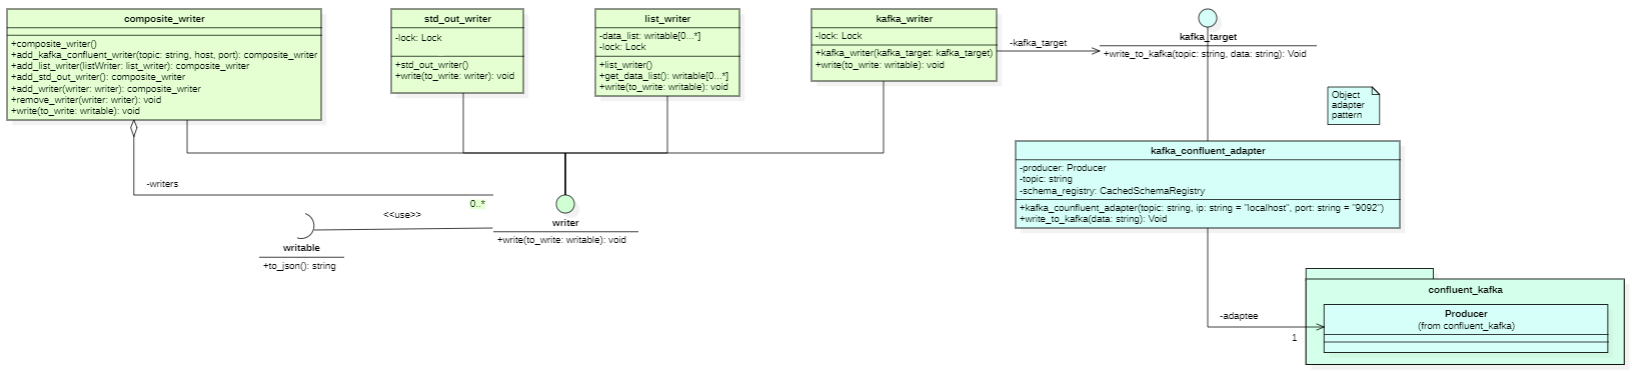
\includegraphics[width=1.1\textwidth]{../Images/SpecificaTecnica/writerModule.PNG}
    \caption{Modulo writers - InnovaCity}
    \label{fig: writersModule}
\end{figure}

Questo modulo si occupa della scrittura e/o invio di informazioni a diverse tipologie di servizi e vuole essere completamentemente indipendendente e non influenzato dal modulo della simulazione dei sensori, così da poter consentire un suo riutilizzo.
Per quanto riguarda la scrittura in Kafka, l'impiego della connessione allo Schema Registry (vedi sezione \S\ref{sec:schema_registry}) consente la convalida del formato del messaggio prima della sua scrittura nei topic Kafka. Questa pratica permette di ridurre il carico di rete nel caso di messaggi malformati, consentendo un filtraggio "alla fonte".

Il modulo è stato progettato per rispettare il Dependecy Inversion Principle \textit{(DIP)}, di conseguenza sia i moduli di alto livello che quelli di basso livello dipendono da astrazioni (interfacce o classi astratte).

\paragraph{Design pattern Strategy + Composite:}
Il modulo presenta un'interfaccia \textit{writer} che offre il metodo di scrittura \textit{write()} di oggetti che implementano \textit{writable}.
Questo metodo è implementato da diverse classi concrete che rappresentano i vari servizi a cui è possibile inviare le informazioni.
L'approccio adottato implementa il design pattern \textit{Strategy} per la scrittura/invio dei dati su diverse piattaforme/servizi e il design pattern \textit{Composite} per la scrittura ad uno o più servizi in modo uniforme.
Nello specifico sono state implentate tre strategie di scrittura: la prima, (\textit{kafka\_writer}), atta a permettere al simulatore di inviare messaggi a topic Kafka,  la seconda (\textit{std\_out\_writer}) atta a permettere di stampare gli \textit{writable} su terminale e la terza (\textit{list\_writer}) per il salvataggio su una lista degli \textit{writable}.
L'utilizzo del design pattern Composite e Strategy in questo caso ha diverse motivazioni:

\begin{enumerate}
    \item \textit{kafka\_writer}, atta a permettere al simulatore di inviare messaggi a Kafka;
    \item \textit{std\_out\_writer}, atta a permettere di stampare i \textit{writable} su terminale;
    \item \textit{list\_writer} per il salvataggio su una lista degli oggetti di tipo \textit{writable}.
\end{enumerate}
L'utilizzo dei design pattern Composite e Strategy in questo caso ha diverse motivazioni:
\begin{itemize}
    \item \textbf{Gestione uniforme dei servizi}: Il pattern Strategy consente di definire una famiglia di algoritmi, incapsularli e renderli intercambiabili. In questo caso, i servizi di scrittura sono trattati come algoritmi intercambiabili, consentendo di scrivere informazioni su diversi servizi senza dover conoscere i dettagli di implementazione di ciascuno.
    \item \textbf{Gestione gerarchica dei servizi}: Il pattern Composite consente di trattare gli oggetti singoli e le loro composizioni (gruppi di oggetti) allo stesso modo. \\
    Nel contesto del modulo, potrebbe esserci la necessità di gestire non solo singoli servizi, ma anche gruppi di servizi. Ad esempio, potrebbe essere utile inviare informazioni al servizio Kafka e contemporaneamente stamparle nel terminale e memorizzarle in un'apposita lista per il testing. Il Composite consente di comporre questi servizi in modo gerarchico e trattarli uniformemente.
\end{itemize}

\paragraph{Design pattern Object Adapter:}
Nello specifico, la classe \textit{kafka\_writer} realizza la sua funzionalità attraverso l'utilizzo del design pattern \textit{Adapter}, nella sua variante \textit{Object Adapter}. Tale scelta è stata motivata dall'impiego della classe \textit{Producer} della libreria \textit{confluent\_kafka}, la quale potrebbe subire variazioni non controllabili da noi. Per garantire la capacità di rispondere prontamente a tali cambiamenti senza dover modificare la classe \textit{kafka\_writer} o altri parti di sistema, si è optato per l'utilizzo di questo pattern, trasferendo così la complessità derivante da tali modifiche proprio nell'adapter.
Inoltre grazie all'interfaccia \textit{kafka\_target}, si è garantita la possibilità di estendere il sistema con nuovi metodi di scrittura su Kafka o l'utilizzo di nuove librerie senza dover modificare la classe \textit{kafka\_writer} ma solamente aggiungendo una nuova classe adapter che implementi \textit{kafka\_target}.

\paragraph{Classi: metodi e attributi}

\begin{itemize}
    \item{\textbf{Interfaccia: \textit{writable}}}
    \begin{itemize}
        \item\textbf{Metodi}: 
        \begin{itemize}
            \item \textbf{to\_json(): string [public, abstract]} - Metodo astratto che deve essere implementato nelle sottoclassi per convertire l'oggetto in una stringa JSON.
        \end{itemize}
        \item\textbf{Note}:
        \begin{itemize}
            \item L'interfaccia \textit{writable} definisce un insieme di metodi che una classe deve implementare perchè possa essere utilizzata dalle strategie di scrittura.
        \end{itemize}
    \end{itemize}
    \item{\textbf{Interfaccia: \textit{writer}}}
     \begin{itemize}
        \item \textbf{Metodi:}
         \begin{itemize}
            \item \textbf{write(to\_write: writable): None [public, abstract]} - Metodo astratto che deve essere implementato nelle sottoclassi per scrivere un oggetto writable.
        \end{itemize}
        \item\textbf{Note}:
        \begin{itemize}
            \item L'interfaccia \textit{writer} definisce il metodo che una classe deve implementare perchè possa essere utilizzata come strategia di scrittura. Rappresenta il componente "\textit{strategy}" del pattern "\textit{Strategy}";
            \item Rappresenta l'interfaccia "\textit{Component}" del pattern \textit{Composite} che descrive le operazioni comuni sia agli elementi semplici che a quelli complessi dell'albero.
        \end{itemize}
    \end{itemize}
    \item{\textbf{Classe: \textit{composite\_writer}}}
    \begin{itemize}
    \item\textbf{Attributi}:
        \begin{itemize}
        \item \textbf{writers: writer [private]} - Lista di oggetti \textit{writer}.
    \end{itemize}
    \item \textbf{Metodi: }
    \begin{itemize}
        \item \textbf{add\_writer(writer: writer ): composite\_writer [public]} - Aggiunge un oggetto che implementa \textit{writer} alla lista writers.
        \item \textbf{add\_kafka\_confluent\_writer(topic: string, host: string, port: int, schema\_registry\_url: string): composite\_writer [public]} - Crea un \textit{kafka\_writer} con un \textit{kafka\_confluent\_adapter} e lo aggiunge alla lista writers. Ritorna se stesso per permettere operazione concatenate.
        \item \textbf{add\_std\_out\_writer(): composite\_writer [public]} - Crea un \textit{std\_out\_writer} e lo aggiunge alla lista writers. Ritorna se stesso per permettere operazione concatenate.
        \item \textbf{add\_list\_writer(writer\_list: list\_writer): composite\_writer [public]} - Aggiunge un \textit{list\_writer} alla lista writers. Ritorna se stesso per permettere operazione concatenate.
        \item \textbf{remove\_writer(writer: writer): composite\_writer [public]} - Rimuove un \textit{writer} dalla lista writers.  Ritorna se stesso per permettere operazione concatenate.
        \item \textbf{write(to\_write: writable): \textit{composite\_writer} [public]} - Chiama il metodo write su ogni writer nella lista writers passando come attributo il \textit{writable} ricevuto.
    \end{itemize}
    \item\textbf{Note}:
        \begin{itemize}
            \item La classe è la componente "Composite" del pattern \textit{Composite}, ovvero l'elemento che può avere sottoelementi;
            \item Dopo aver ricevuto una richiesta, il contenitore (detto composite) delega il lavoro ai suoi sottoelementi: foglie o altri contenitori.
        \end{itemize}
    \end{itemize}
    \item{\textbf{Classe: \textit{std\_out\_writer}}}
    \begin{itemize}
    \item\textbf{Attributi}:
        \begin{itemize}
        \item \textbf{lock:threading.Lock [private]} - Lock per garantire l'accesso esclusivo alla stampa ed un esecuzione Thread safe.
    \end{itemize}
    \item \textbf{Metodi: }
    \begin{itemize}
        \item \textbf{write(to\_write: writable): None [public]} - Stampa l'oggetto writable come stringa JSON nella console;
    \end{itemize}
    \item\textbf{Note}:
        \begin{itemize}
            \item La classe è una strategia di scrittura del pattern \textit{Strategy} ma anche la componente "Leaf" del pattern \textit{Composite}, ovvero l'elemento base che non ha sottoelementi.
        \end{itemize}
    \end{itemize}
    \item{\textbf{Classe: \textit{list\_writer}}}
    \begin{itemize}
    \item\textbf{Attributi}:
        \begin{itemize}
        \item \textbf{data\_list:list [private]} - Lista per memorizzare gli oggetti writable.
        \item \textbf{lock:threading.Lock [private]} - Lock per garantire l'accesso esclusivo alla lista ed un esecuzione Thread safe.
    \end{itemize}
    \item \textbf{Metodi: }
    \begin{itemize}
        \item \textbf{write(to\_write: writable): None [public]} - Aggiunge l'oggetto writable alla lista.
        \item \textbf{get\_data\_list(): list [public]} - Restituisce la lista di oggetti writable.
    \end{itemize}
    \item\textbf{Note}:
        \begin{itemize}
            \item La classe è una strategia di scrittura del pattern \textit{Strategy} ma anche la componente "Leaf" del pattern \textit{Composite}, ovvero l'elemento base che non ha sottoelementi.
        \end{itemize}
    \end{itemize}
    \item{\textbf{Classe: \textit{kafka\_writer}}}
    \begin{itemize}
    \item\textbf{Attributi}:
        \begin{itemize}
        \item \textbf{lock:threading.Lock [private]} - Lock per garantire l'accesso esclusivo alla scrittura su Kafka ed un esecuzione Thread safe.
        \item \textbf{kafka\_target:kafka\_target [private]} - Riferimento ad un implementazione di kafka\_target per effettuare l'effettiva scrittura in Kafka tramite librerie.
    \end{itemize}
    \item \textbf{Metodi: }
    \begin{itemize}
        \item \textbf{write(to\_write: writable): None [public]} - Scrive l'oggetto \textit{writable} come stringa JSON su Kafka.
    \end{itemize}
    \item\textbf{Note}:
        \begin{itemize}
            \item La classe è una strategia di scrittura del pattern \textit{Strategy} ma anche la componente "Leaf" del pattern \textit{Composite}, ovvero l'elemento base che non ha sottoelementi.
            \item La costruzione dell'oggetto \textit{kafka\_writer} richiede un riferimento ad un oggetto che implementi l'interfaccia kafka\_target.
        \end{itemize}
    \end{itemize}
    \item{\textbf{Interfaccia: kafka\_target}}
    \begin{itemize}
        \item \textbf{Metodi: }
        \begin{itemize}
            \item \textbf{write\_to\_kafka(data: string): None [public, abstract]} - Metodo astratto che deve essere implementato nelle sottoclassi per scrivere dati su Kafka.
        \end{itemize}
        \item\textbf{Note}:
        \begin{itemize}
            \item La classe è una interfaccia che fornisce un contratto per le operazioni di scrittura/invio a topic Kafka.
            \item Rappresenta il componente Target del pattern \textit{Object Adapter}.
        \end{itemize}
    \end{itemize}
    \item{\textbf{Classe: \textit{KafkaConfluentAdapter}}}
    \begin{itemize}
        \item\textbf{Attributi}:
        \begin{itemize}
            \item \textbf{topic:string [private]} - Il topic su cui scrivere in Kafka;
            \item \textbf{producer:Producer [private]} - Il producer Kafka per inviare messaggi;
            \item \textbf{schema\_registry:CachedSchemaRegistryClient [private]} - Consente di interagire con Confluent Schema Registry in modo efficiente, memorizza in cache gli schemi recuperati da Schema Registry, riducendo le chiamate di rete e migliorando la velocità di accesso agli schemi.
        \end{itemize}
    \end{itemize}
    \item \textbf{Metodi: }
    \begin{itemize}
        \item \textbf{write\_to\_kafka(data: string): None [public]} - Scrive i dati su Kafka dopo averli validati rispetto allo schema registrato per il topic di destinazione.
    \item\textbf{Note}:
        \begin{itemize}
            \item La classe è un'implementazione concreta dell'interfaccia \textit{kafka\_target}, utilizzando la libreria \textit{confluent-kafka} per interagire con Kafka;
            \item Rappresenta il componente "Adapter" del pattern \textit{Object Adapter};
            \item Il Producer kafka rappresenta la componente "service" del pattern \textit{Object Adapter};
            \item Prima di inviare il messaggio (ovvero la misurazione) controlla che sia nel formato/schema corretto per il topic di destinazione evintando cosi sovraccarico inutile di rete;
            \item Nel caso in cui il formato del messaggio sia scorretto questo viene scartato.
        \end{itemize}
    \end{itemize}
\end{itemize}

\subsubsection{Modulo Threading/Scheduling}
\begin{figure}[H]
    \centering
    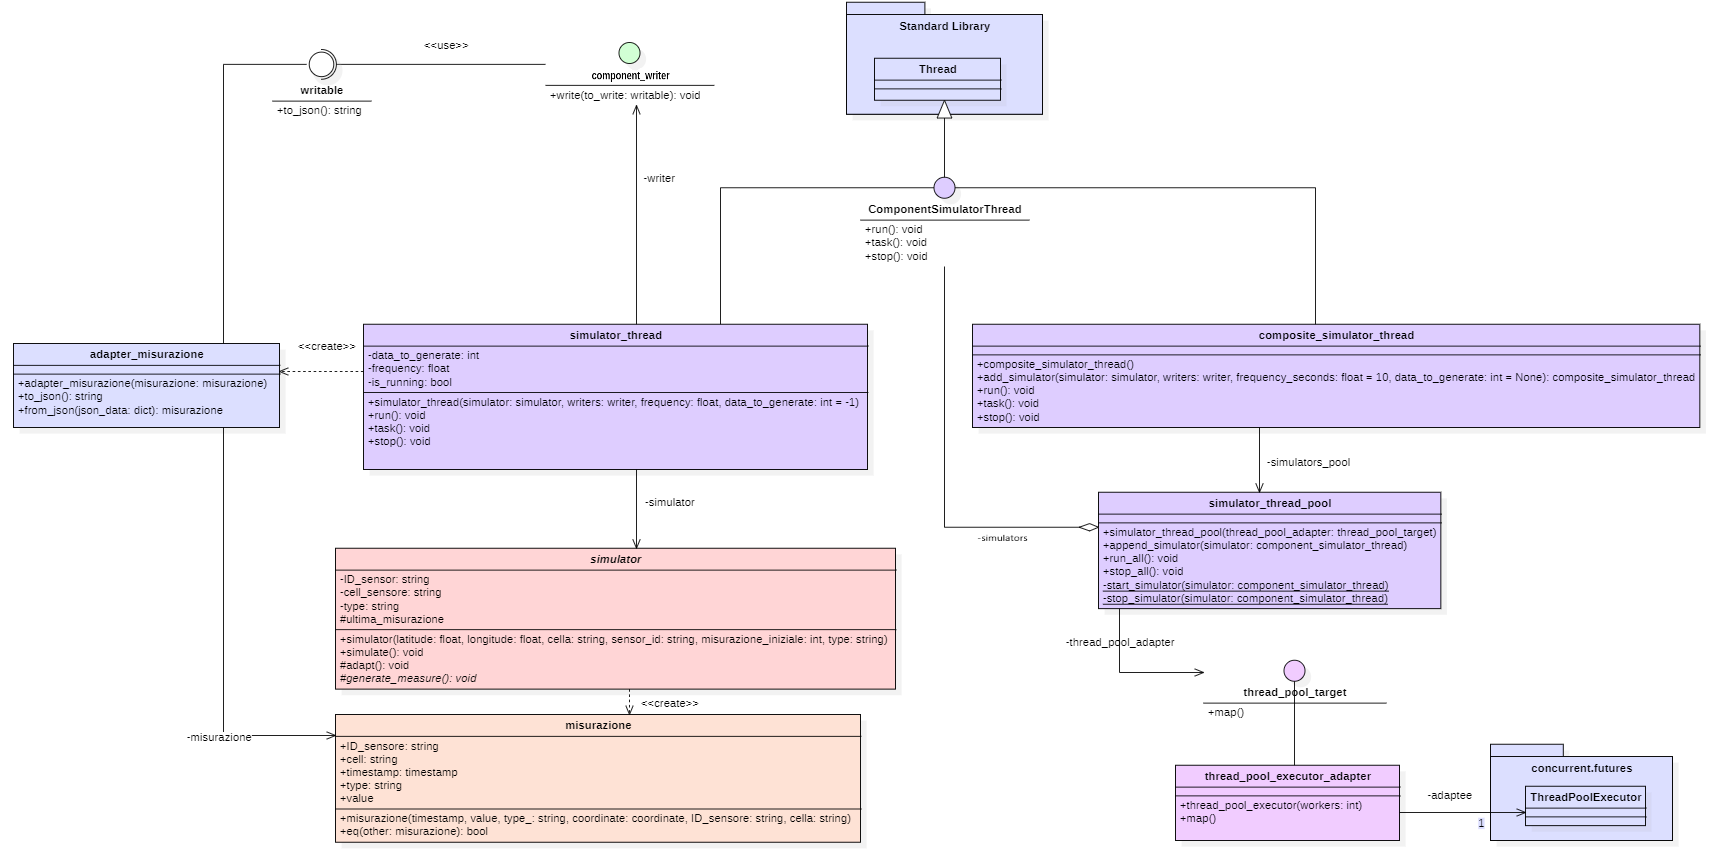
\includegraphics[width=1.1\textwidth]{../Images/SpecificaTecnica/simulatorThread.PNG}
    \caption{Modulo Threading/Scheduling simulatori sensori - InnovaCity}
    \label{fig: Modulo_simulatori_sensori_thread}
\end{figure}
Questo modulo si propone di gestire la logica di pianificazione per il recupero dei dati dai simulatori dei sensori e di inviare/scrivere tali dati utilizzando il modulo Writer.

Funge da orchestratore per i due moduli appena descritti, offrendo la possibilità di configurare la frequenza di campionamento e il numero di misurazioni da eseguire.

Inoltre, incorpora una logica di ottimizzazione, simile a quella impiegata dai microcontrollori dei sensori nella realtà, al fine di evitare la trasmissione di dati ridondanti, inviando solo i cambiamenti di stato dei sensori.

Il modulo è stato progettato per rispettare il Dependecy Inversion Principle \textit{(DIP)}, di conseguenza sia i moduli di alto livello che quelli di basso livello dipendono da astrazioni (interfacce o classi astratte).

\paragraph{Design pattern Composite:}
Come il modulo di scrittura anche questo è sviluppato secondo il pattern \textit{Composite} che permette di gestire un singolo thread di esecuzione o un gruppo di thread in modo uniforme.

\paragraph{Design pattern Object Adapter:}
Inoltre, considerando l'impiego di più thread per un esecuzione parallela, per delegare l'orchestrazione delle operazioni, si è deciso di utilizzare delle ThreadPool.

Al fine di evitare modifiche dirette al codice di \textit{simulator\_thread\_pool}, è stato adottato il pattern \textit{Object Adapter} per adattare la ThreadPool di Python a un'interfaccia comune con cui \textit{simulator\_thread\_pool} possa interagire.

Questo approccio consente di modificare la logica o la libreria utilizzata per la gestione dei thread senza richiedere modifiche al codice di \textit{simulator\_thread\_pool}, ma semplicemente aggiungendo una nuova classe adapter che implementi \textit{thread\_pool\_target}.

Un'altra implementazione del pattern \textit{Object Adapter} viene impiegata per adattare gli oggetti \textit{misurazione} del modulo dei Simulatori all'interfaccia \textit{writable} del modulo Writers. La classe \textit{adapter\_misurazione}, implementando l'interfaccia \textit{writable}, fornisce un'implementazione del metodo \textit{to\_json()} che consente di convertire un oggetto \textit{misurazione} nel formato JSON, compatibile con il formato definito nello Schema Registry e riconosciuto da Kafka.
\ref*{sec:formatoMessaggi}

\paragraph{Classi, interfacce, metodi e attributi}

\begin{itemize}
    \item{\textbf{Interfaccia: \textit{component\_simulator\_thread}}}
    \begin{itemize}
        \item \textbf{Metodi:}
        \begin{itemize}
            \item \textbf{run(): None [public, abstract]} - Metodo astratto che deve essere implementato nelle sottoclassi per definire il comportamento del thread quando viene avviato;
            \item \textbf{task(): None [public, abstract]} - Metodo astratto che deve essere implementato nelle sottoclassi per definire il compito specifico che il thread deve eseguire;
            \item \textbf{stop(): None [public, abstract]} - Metodo astratto che deve essere implementato nelle sottoclassi per definire come fermare il thread.
        \end{itemize}
        \item\textbf{Note}:
        \begin{itemize}
            \item Eredita le proprietà e i metodi della classe \textit{Thread} della \textit{Standard Library};
            \item \textit{component\_simulator\_thread} è un interfaccia di threading per la simulazione dei sensori, fornisce un contratto per le operazioni di avvio, esecuzione del compito e arresto;
            \item Rappresenta il componente "Component" del pattern \textit{Composite}, descrive le operazioni comuni sia ai singoli Thread sia a composizioni di questi;
            \item L'utilizzatore dei simulatori può lavorare allo stesso modo con elementi semplici (singoli Thread) o complessi (insiemi di Thread in forma di albero).
        \end{itemize}
    \end{itemize}
    \item{\textbf{Classe: \textit{simulator\_thread}}}
    \begin{itemize}
        \item\textbf{Attributi}:
        \begin{itemize}
            \item \textbf{simulator: \textit{simulator} [private]} - Il simulatore da utilizzare per generare i dati;
            \item \textbf{frequency: float [private]} - La frequenza con cui generare i dati;
            \item \textbf{is\_running: bool [private]} - Flag per controllare se il thread è in esecuzione;
            \item \textbf{data\_to\_generate: int [private]} - Il numero di dati da generare;
            \item \textbf{writers: writer [private]} - L'oggetto implementazione di \textit{writer} per scrivere i dati generati. (Singolo o albero - Composite pattern)
        \end{itemize}

        \item \textbf{Metodi:}
        \begin{itemize}
            \item \textbf{run(): None [public]} - Avvia il thread del simulatore;
            \item \textbf{task(): None [public]} - Definisce il compito specifico che il thread deve eseguire, contiene la logica per generare il numero di misurazioni richieste con l'intervallo specificato alla costruzione.
            Inoltre evita l'invio di misurazioni consecutive uguali cosi da ridurre il carico scartando dati ridondanti e deducibili inviando ai \textit{Writers} solo i cambi di stato del sensore da cui acquisisce la misurazione.
            All'interno del metodo, la misurazione restituita dal simulatore, viene adattata ad un oggetto \textit{writable} tramite \textit{adapter\_misurazione} ed inviata ai \textit{Writers};
            \item \textbf{stop(): None [public]} - Ferma il thread del simulatore.
        \end{itemize}
        \item\textbf{Note}:
        \begin{itemize}
            \item La classe è un'implementazione concreta dell'interfaccia \textit{component\_simulator\_thread};
            \item Utilizza un oggetto \textit{\textit{simulator}} per generare dati a una certa frequenza e un oggetto che implementa\textit{component\_writer} per scrivere i dati generati;
            \item Rappresenta il componente Leaf del pattern \textit{Composite};
            \item Se \textit{data\_to\_generate} < 0, allora genera misurazioni finchè il thread non viene interroto dall'esterno;
            \item Sebbene i simulatori non siano considerati dalla proponente parte del prodotto, la logica di ottimizzazione per inviare solo i cambi di stato dei sensori viene implementata nella realtà IoT.
            
            Di conseguenza, è stata presa la decisione di replicarla. È importante notare che questa logica non è incorporata nel simulatore del sensore, il quale ha unicamente il compito semantico di generare dati come un vero sensore. Invece, essa è implementata in \textit{simulator\_thread}, il quale agisce in modo simile a un microcontrollore, responsabile sia della gestione dell'intervallo di campionamento che della logica per l'invio delle misurazioni;
            \item Nel corso dello sviluppo futuro, potrebbe risultare vantaggioso considerare l'implementazione di un pattern \textit{Strategy} per gestire la strategia/criterio di invio dei dati, che possa distinguere tra un invio continuo e la trasmissione solo in caso di cambiamenti di stato. Tuttavia, al momento della decisione, si è optato per non includerlo al fine di evitare un'eccessiva complessità nell'architettura, nota come sovraingegnerizzazione. Tale scelta è stata dettata dalla volontà di mantenere un equilibrio tra la completezza del sistema e la sua semplicità, favorendo un'implementazione più diretta e immediata delle funzionalità richieste.
        \end{itemize}
    \end{itemize}

    \item{\textbf{Classe: \textit{adapter\_misurazione}}}
    \begin{itemize}
        \item\textbf{Attributi}:
        \begin{itemize}
            \item \textbf{misurazione: \textit{misurazione} [private]} - L'oggetto \textit{misurazione} da adattare.
        \end{itemize}
        \item \textbf{Metodi: }
        \begin{itemize}
            \item \textbf{to\_json(): string [public]} - Converte l'oggetto \textit{misurazione} in una stringa JSON conforme a quanto definito in \ref{sec:formatoMessaggi};
            \item \textbf{from\_json(json\_data: dict): misurazione [staticmethod, public]} - Crea un oggetto \textit{misurazione} da un dizionario JSON.
        \end{itemize}
        \item\textbf{Note}:
        \begin{itemize}
            \item La classe è un'implementazione concreta dell'interfaccia \textit{writable}. Fornisce metodi per convertire un oggetto \textit{misurazione} in un formato JSON e viceversa;
            \item Rappresenta la componente "Adapter" del pattern \textit{Object Adapter}.
        \end{itemize}
    \end{itemize}

    \item{\textbf{Classe: \textit{composite\_simulator\_thread}}}
    \begin{itemize}
        \item\textbf{Attributi}:
        \begin{itemize}
            \item \textbf{simulator\_executor: simulator\_thread\_pool [private]} - L'executor per gestire l'esecuzione di più thread dei simulatori.
        \end{itemize}
        \item \textbf{Metodi: }
        \begin{itemize}
            \item \textbf{add\_simulator(simulator: simulator, writers: component\_writer, frequency: float, data\_to\_generate: int): composite\_simulator\_thread [public]} - Aggiunge un simulatore all'executor;
            \item \textbf{add\_simulator\_thread(thread\_simulator: component\_simulator\_thread): composite\_simulator\_thread [public]} - Aggiunge un \textit{simulator\_thread} all'executor;
            \item \textbf{run(): None [public]} - Avvia tutti i \textit{simulator\_thread} nell'executor;
            \item \textbf{stop(): None [public]} - Ferma tutti i \textit{simulator\_thread} nell'executor;
            \item \textbf{task(): None [public]} - Avvia tutti i \textit{simulator\_thread} nell'executor.
        \end{itemize}
        \item\textbf{Note}:
        \begin{itemize}
            \item La classe è un'implementazione concreta dell'interfaccia \textit{component\_simulator\_thread}, utilizza un oggetto \textit{simulator\_thread\_pool} per gestire l'esecuzione di vari simulatori;
            \item Rappresenta il componente "Composite" del pattern \textit{Composite}.
            \item Utilizzando il metodo \textit{run()} viene creato un nuovo thread che permette di eseguire la funzione \textit{task()} in modo sincrono.
            \item Utilizzando il metodo \textit{task()} direttamente non è possibile avere un'esecuzione asincrona. La funzione \textit{task()} viene eseguita sul thread chiamante, bloccando l'esecuzione del codice fino al termine della sua esecuzione. Questa funzione viene utilizzata dalle ThreadPool che creano dei thread per l'esecuzione asincrona delle task.
        \end{itemize}
    \end{itemize}

    \item{\textbf{Classe: \textit{simulator\_thread\_pool}}}
    \begin{itemize}
        \item\textbf{Attributi:}
        \begin{itemize}
            \item \textbf{simulators: List[component\_simulator\_thread] [private]} - La lista dei \textit{component\_simulator\_thread} da eseguire (Singoli thread o alberi di thread);
            \item \textbf{thread\_pool\_adapter: thread\_pool\_target [private]} - Thread pool per gestire l'esecuzione parallela dei simulatori.
        \end{itemize}
        \item \textbf{Metodi:}
        \begin{itemize}
            \item \textbf{run\_all(): None [public]} - Avvia tutti i simulatori nella thread pool, utilizzando l'interfaccia fornita da \textit{thread\_pool\_target} per l'esecuzione controllata di attività in parallelo.
            Per farlo viene utilizzato il metodo \textit{map()} di \textit{thread\_pool\_target} per mappare la funzione statica \textit{start\_simulator()} su ogni \textit{component\_simulator\_thread} in \textit{simulators};
            \item \textbf{stop\_all(): None [public]} - Ferma tutti i simulatori nel thread pool, utilizzando l'interfaccia fornita da \textit{thread\_pool\_target} per l'esecuzione controllata di attività in parallelo.
            Per farlo utilizza il metodo \textit{map()} di \textit{thread\_pool\_target} per mappare la funzione statica \textit{stop\_simulator()} su ogni \textit{component\_simulator\_thread} in \textit{simulators};
            \item \textbf{append\_simulator(simulator: component\_simulator\_thread): None [public]} - Aggiunge un \textit{component\_simulator\_thread} alla threadpool;
            \item \textbf{start\_simulator(simulator: component\_simulator\_thread): None [private, static]} - Avvia un \textit{component\_simulator\_thread};
            \item \textbf{stop\_simulator(simulator: component\_simulator\_thread): None [private, static]} - Ferma un \textit{component\_simulator\_thread}.
        \end{itemize}
        \item\textbf{Note}:
        \begin{itemize}
            \item La classe gestisce una pool di thread per l'esecuzione di vari simulatori, utilizzando un oggetto che implementa \textit{thread\_pool\_target} per gestire l'esecuzione dei simulatori;
            \item I metodi \textit{run\_all()} e \textit{stop\_all()} utilizzano l'interfaccia fornita da \textit{thread\_pool\_target} per mappare rispettivamente la funzione statica \textit{start\_simulator()} e \textit{stop\_simulator()} per ogni \textit{component\_simulator\_thread} in \textit{simulators};
            \item Grazie all'utilizzo di \textit{thread\_pool\_target} è possibile estendere il sistema con nuovi metodi o utilizzare nuove librerie senza dover modificare la classe \textit{simulator\_thread\_pool}, ma solamente aggiungendo una nuova classe adapter che implementi \textit{thread\_pool\_target}.
        \end{itemize}
    \end{itemize}

    \item{\textbf{Interfaccia: \textit{thread\_pool\_target}}}
    \begin{itemize}
        \item\textbf{Metodi:}
        \begin{itemize}
            \item \textbf{map(func, iterable): [abstractmethod]} - Un metodo astratto che deve essere implementato nelle classi derivate. Questo metodo applica la funzione \textit{func} a ogni elemento nell'\textit{iterable}.
        \end{itemize}
        \item\textbf{Note}:
        \begin{itemize}
            \item L'interfaccia rappresenta la componente "Target" del pattern \textit{Object Adapter} fornendo un contratto per le operazioni di esecuzione controllata di attività in parallelo.
        \end{itemize}
    \end{itemize}

    \item{\textbf{Classe: \textit{thred\_pool\_executor\_adapter}}}
    \begin{itemize}
        \item\textbf{Attributi:}
        \begin{itemize}
            \item \textbf{executor: concurrent.futures.ThreadPoolExecutor [private]} - L'executor della thread pool per gestire l'esecuzione dei thread dalla libreria \textit{concurrent.futures}. 
        \end{itemize}
        \item \textbf{Metodi:}
        \begin{itemize}
            \item \textbf{map(func, iterable): [public]} - Applica la funzione \textit{func} a ogni elemento nell'\textit{iterable} utilizzando l'executor del thread pool (\textit{executor}).
        \end{itemize}
        \item\textbf{Note}:
        \begin{itemize}
            \item La classe è un'implementazione concreta dell'interfaccia \textit{thread\_pool\_target}, utilizzando un oggetto \textit{concurrent.futures.ThreadPoolExecutor} per gestire l'esecuzione dei thread;
            \item Rappresenta il componente "Adapter" del pattern \textit{Object Adapter};
            \item Adatta l'oggetto ThreadPoolExecutor dalla libreria \textit{concurrent.futures};
            \item Al momento della costruzione deve essere fornito il parametro intero "workers" ovvero
            Il numero massimo di thread che è possibile utilizzare per eseguire le task indicate.
        \end{itemize}
    \end{itemize}
\end{itemize}

\subsubsection{Progettazione - Panoramica UML }
\begin{figure}[H]
    \centering
    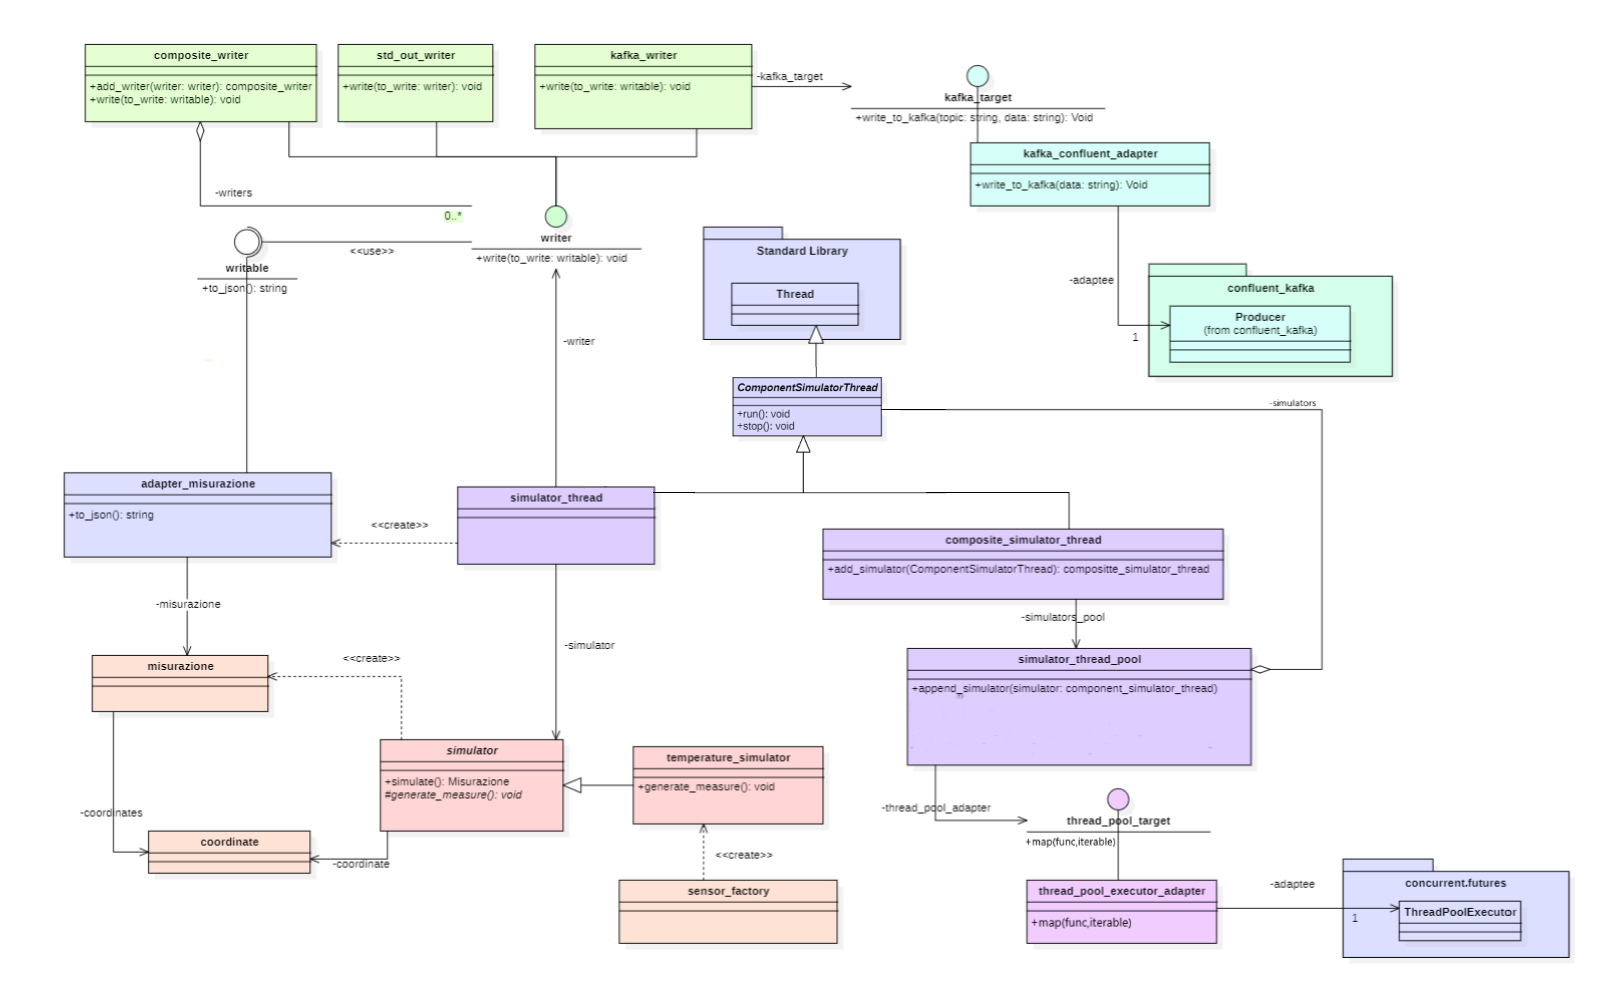
\includegraphics[width=1.1\textwidth]{../Images/SpecificaTecnica/progettazioneCompSimulatori.PNG}
    \caption{Panoramica progettazione simulatori sensori UML - InnovaCity}
    \label{fig: panor_sim}
\end{figure}
L'immagine vuole mostrare sinteticamente la struttura dei moduli Simulatori, Writers e Threading/Scheduling e le relazioni tra le classi principali di questi moduli.

In particolare, si evidenzia la presenza del pattern \textit{Composite} per la gestione di più servizi di scrittura e di più thread di esecuzione, il pattern \textit{Strategy} per la scrittura su diversi servizi e il pattern \textit{Object Adapter} per adattare le ThreadPool di Python e gli oggetti \textit{misurazione} ai \textit{writer}.

Viene riportato solo il sensore di temperatura come implementazione concreta di \textit{simulator} in quanto le altre implementazioni sono analoghe.